\documentclass[12pt]{article}
\usepackage{homework}
\usepackage{tikz}
\usepackage{pgfplots}
\pagestyle{fancy}

% assignment information
\def\course{Vacation Work}
\def\assignmentno{Problem Sheet B}
\def\assignmentname{Calculus}
\def\name{Xin, Wenkang}
\def\time{September 22, 2022}

\begin{document}

\begin{titlepage}
    \begin{center}
        \large
        \textbf{\course}

        \vfill

        \Huge
        \textbf{\assignmentno}

        \vspace{1.5cm}

        \large{\assignmentname}

        \vfill

        \large
        \name

        \time
    \end{center}
\end{titlepage}


%==========
\pagebreak
\section*{Differentiation}
%==========


\problem{1}{}

\subproblem{a}
\begin{equation}
    \deri{}{x} (x^{2} \sin{x} + \ln{x}) = 2x \sin{x} + x^{2} \cos{x} + \frac{1}{x}
\end{equation}

\subproblem{b}
\begin{equation}
    \deri{}{x} \left( \frac{1}{\sin{x}} \right) = -\frac{\cos{x}}{\sin^{2}{x}}
\end{equation}

\subproblem{c}
\begin{equation}
    \deri{}{x} (2^{x}) = \deri{}{x} (e^{x\ln{2}}) = \ln{2} (e^{x\ln{2}})
\end{equation}
\qed


\problem{2}{}

\subproblem{a}
\begin{equation}
    F'(x) = 3\cos{x} - 4\sin{x}
\end{equation}

\begin{equation}
    F''(x) = -3\sin{x} - 4\cos{x}
\end{equation}

\subproblem{b}
\begin{equation}
    y' = \frac{1}{x}
\end{equation}

\begin{equation}
    y'' = - \frac{1}{x^2}
\end{equation}
\qed


\problem{3}{}
Given the parametric equations of $x$ and $y$ in terms of $\theta$, we have by chain rule:

\begin{equation}
    \deri{y}{x} = \deri{y}{\theta} / \deri{x}{\theta} = \frac{1 - \cos{\theta}}{\sin{\theta}}
\end{equation}

A further differentiation by chain rule yields:

\begin{equation}
    \begin{split}
        \deri[2]{y}{x} &= \deri{}{x} \left( \deri{y}{x} \right) \\
        &= \deri{}{\theta} \left( \deri{y}{x} \right) \deri{\theta}{x} \\
        &= \frac{\sin{\theta} \sin{\theta} - \cos{\theta}(1 - \cos{\theta})}{\sin^{2}{\theta}} \frac{1}{a(1 - \cos{\theta})} \\
        &= \frac{1}{a \sin^{2}{\theta}}
    \end{split}
\end{equation}
\qed


%==========
\pagebreak
\section*{Stationary points and graph sketching}
%==========


\problem{4}{}
To find the stationary points of $E(r)$, differentiate it once to yield:

\begin{equation}
    E'(r) = \frac{(1+r)^{2} (4) - 2(1+r)(4r)}{(1+r)^{4}} = \frac{4 - 4r^{2}}{(1+r)^{4}}
\end{equation}

This leads to two stationary points at $r = 1$ and $r = -1$, but the function has a singularity at $r = -1$ so it is discarded. Differentiating further:

\begin{equation}
    E''(r) = \frac{(1+r)^{4} (-8r) - 4(1+r)^{3}(4-4r^{2})}{(1+r)^{8}} = \frac{8r - 16}{(1+r)^{4}}
\end{equation}

Since $E''(1) < 0$, and $r = 1$ is a local maximum.

\begin{center}
    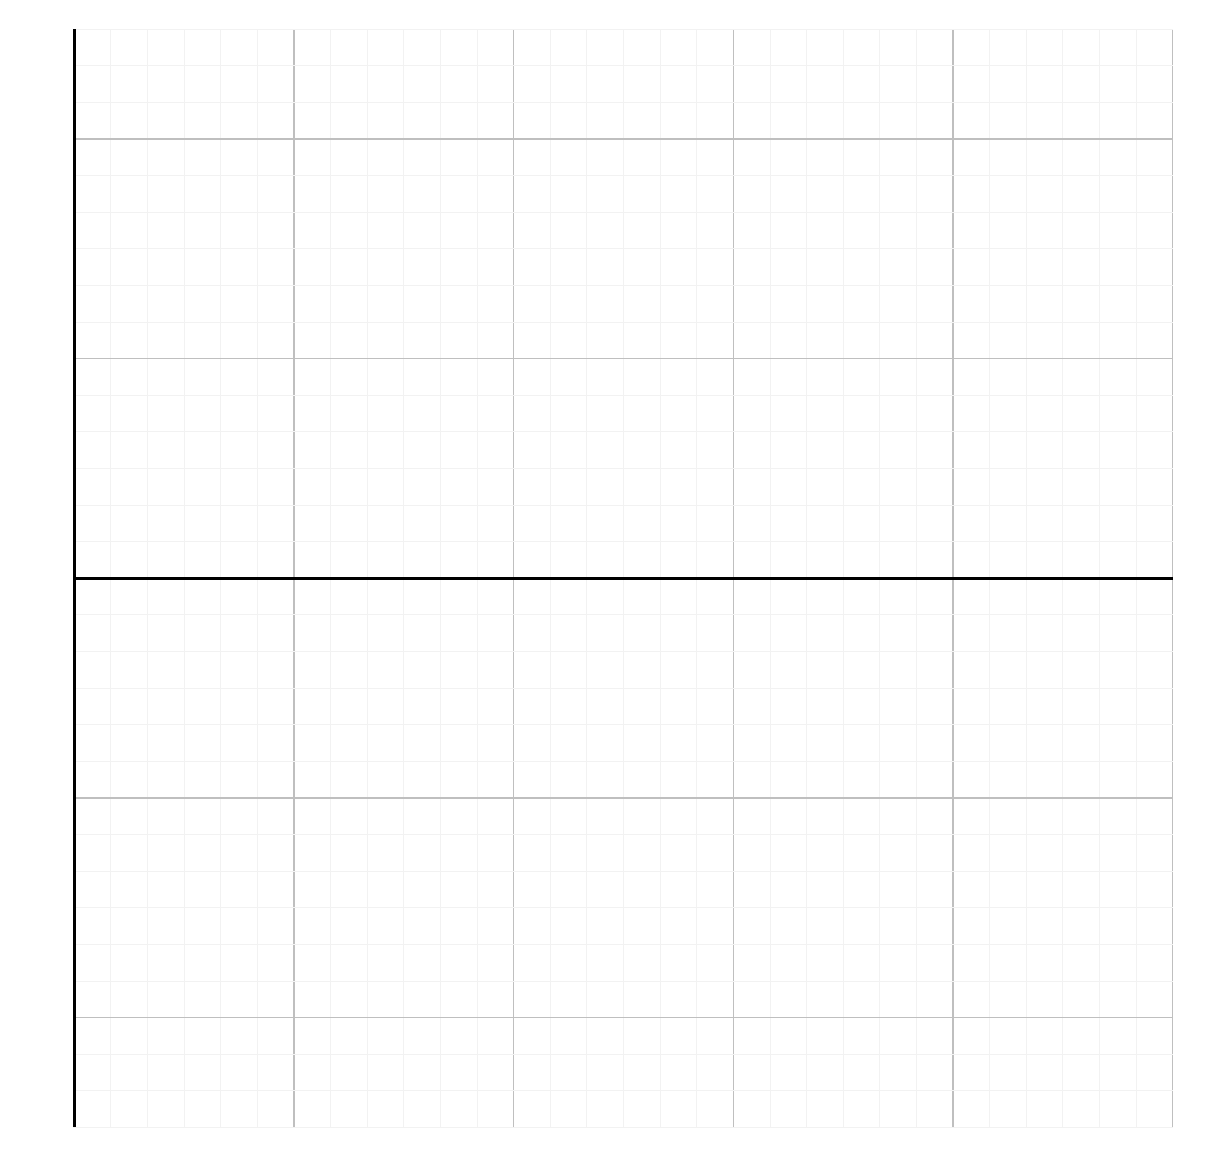
\begin{tikzpicture}[scale = 2.45]
        \begin{axis}[
                xmin=0,xmax=10,
                ymin=-5,ymax=5,
                grid=both,
                grid style={line width=.1pt, draw=gray!10},
                major grid style={line width=.2pt,draw=gray!50},
                axis lines*=middle,
                minor tick num=5,
                xtick style={draw=none},ytick style={draw=none},
                xticklabels={,,},yticklabels={,,},
                axis equal image
            ]
        \end{axis}
    \end{tikzpicture}
\end{center}
\qed


%==========
\pagebreak
\section*{Hyperbolic functions}
%==========


\problem{5}{}

\qed


\problem{6}{}
From the definitions of $\sinh{x}$ and $\tanh{x}$:

\begin{equation}
    \deri{}{x} (\sinh{x}) = \deri{}{x} \left( \frac{e^{x} - e^{-x}}{2} \right) = \frac{e^{x} + e^{-x}}{2} = \cosh{x}
\end{equation}

\begin{equation}
    \deri{}{x} (\tanh{x}) = \deri{}{x} \left( \frac{e^{x} - e^{-x}}{e^{x} + e^{-x}} \right) = \frac{(e^{x} + e^{-x})^{2} - (e^{x} - e^{-x})^{2}}{(e^{x} + e^{-x})^{2}} = \left( \frac{1}{\cosh{x}} \right)^{2}
\end{equation}
\qed


%==========
\pagebreak
\section*{Integration}
%==========


\problem{7}{}

\subproblem{a}
\begin{equation}
    \int 1 + 2x + 3x^{2} \diff{x} = x + x^{2} + x^{3} + C
\end{equation}

\subproblem{b}
\begin{equation}
    \int \sin{2x} - \cos{3x} \diff{x} = - \frac{1}{2} \cos{2x} - \frac{1}{3} \sin{3x} + C
\end{equation}

\subproblem{c}
\begin{equation}
    \int e^{t} + \frac{1}{t^{2}} \diff{t} = e^{t} - \frac{1}{t} + C
\end{equation}

\subproblem{d}
\begin{equation}
    \int  \diff{\omega} = \omega + C
\end{equation}

where all the $C$ above are arbitrary constants.
\qed


\problem{8}{}

\subproblem{a}
\begin{equation}
    \int_{-1/4}^{1/4} \cos{(2\pi x)} \diff{x} = \frac{1}{2\pi} \sin{(2\pi x)} \rvert_{-1/4}^{1/4} = \frac{1}{\pi}
\end{equation}

\subproblem{b}
\begin{equation}
    \int_{0}^{3} (2t - 1)^{2} \diff{t} = \frac{1}{6} (2t - 1)^{3} \rvert_{0}^{3} = 21
\end{equation}

\subproblem{c}
\begin{equation}
    \int_{1}^{2} \frac{(1 + e^{t})^{2}}{e^{t}} \diff{t} = \int_{1}^{2} e^{t} + 2 + e^{-t} \diff{t} = (e^{t} - e^{-t} + 2t) \rvert_{1}^{2} = e^{2}  - \frac{1}{e^{2}} - e + \frac{1}{e} + 2
\end{equation}

\subproblem{d}
\begin{equation}
    \int_{4}^{9} \sqrt{x}(x - \frac{1}{x}) \diff{x} = (\frac{2}{5} x^{5/2} - 2 x^{1/2}) \rvert_{4}^{9} = \frac{412}{5}
\end{equation}

\subproblem{e}
$x^{3}$ is an odd function as $x^{3} = -(-x)^{3}$, so the definite integral equals zero.
\qed


\problem{9}{}
Integrating by parts:

\begin{equation}
    \begin{split}
        \int x^{2} e^{-x} \diff{x} &= - x^{2} e^{-x} + \int 2x e^{-x} \diff{x} \\
        &= - x^{2} e^{-x} - 2x e^{-x} + \int 2e^{-x} \diff{x} \\
        &= - x^{2} e^{-x} - 2x e^{-x} - 2e^{x} + C
    \end{split}
\end{equation}

where $C$ is an arbitrary constant.
\qed


\problem{10}{}
The integral is a standard form:

\begin{equation}
    \int \sin{x} (1+\cos{x})^{4} \diff{x} = -\frac{1}{5} (1 + \cos{x})^{5} + C
\end{equation}

where $C$ is an arbitrary constant.
\qed


\problem{11}{}
For the two curves to meet each other:

\begin{equation}
    \begin{split}
        x^{2} + 2 &= 5 - 2x \\
        x^{2} + 2x - 3 &= 0 \\
        (x + 3)(x - 1) &= 0
    \end{split}
\end{equation}

Thus the integration takes place in the interval $[-3, 1]$. The sought area is thus:

\begin{equation}
    \begin{split}
        &\left\lvert \int_{-3}^{1} x^2 + 2 - (5 - 2x) \diff{x} \right\rvert \\
        =&\left\lvert \int_{-3}^{1} x^{2} + 2x - 3 \diff{x} \right\rvert \\
        =&\boxed{\frac{32}{3}}
    \end{split}
\end{equation}
\qed


\problem{12}{}

\subproblem{a}
Slicing the volume of revolution into infinitesimal disks, each of radius $y = f(x)$, thickness $\dd{x}$ and thus volume $\dd{V} = \pi y^{2} \dd{x}$, the total volume of revolution $V$ from $a$ to $b$ is represented by the integral:

\begin{equation}
    V = \int \diff{V} = \int_{a}^{b} \pi f(x)^{2} \diff{x}
\end{equation}

For the function $y = \frac{1}{x}$, the volume of revolution from $1$ to $\infty$ is represented by the improper integral:

\begin{equation}
    \begin{split}
        V &= \lim_{n \to \infty} \int_{1}^{n} \pi \frac{1}{x^{2}} \diff{x} \\
        &= \pi \lim_{n \to \infty} \left( -\frac{1}{x} \right) \rvert_{1}^{n} \\
        &= \pi \lim_{n \to \infty} \left( 1 - \frac{1}{n} \right) \\
        &= \boxed{\pi \text{ units}^{3}}
    \end{split}
\end{equation}

\subproblem{b}
By the definition of work done:

\begin{equation}
    W = \int \diff{W} = \int F \diff{x} = \int_{0}^{l} k x^{2} \diff{x} = \frac{1}{3} k l^{3}
\end{equation}
\qed


\end{document}